\documentclass[11pt]{article}
\usepackage[margin=1in]{geometry}
\usepackage{graphicx}
\usepackage{enumitem}
\usepackage{hyperref}

\title{Project 3 Report --- Group10}
\author{Muhan Zhang \and Danhua Zhao}
\date{}

\begin{document}
\maketitle

\section*{Team \& Repo}
\begin{itemize}[leftmargin=*]
  \item Group: 10
  \item Members: Muhan Zhang, Danhua Zhao
  \item Division of work: Muhan Zhang (2PC, Raft core, Docker), Danhua Zhao (testing, logs/screenshots, report)
  \item Base repo: \url{https://github.com/J1anXu/Distributed-picture-sharing-system}
  \item Submission repo:\\ \url{https://github.com/ricolalemon/-Distributed-picture-sharing-system-consensus}
  \item Consensus additions: \texttt{consensus\_node/}, \texttt{docker-compose-consensus.yml}
\end{itemize}

\section*{Overview}
Added a 5-node consensus cluster with Two-Phase Commit (vote+decision) and Raft (leader election, heartbeats, log replication). Followers forward client commands to the leader; majority commit persists state to \texttt{/data/consensus\_store.json}.

\section*{Architecture Highlights}
\begin{itemize}[leftmargin=*]
  \item Heartbeat: 1s; Election timeout: randomized 1.5--3s.
  \item Full-log replication on AppendEntries; majority ACK triggers commit.
  \item Protos: \texttt{consensus\_node/two\_phase.proto}, \texttt{consensus\_node/raft.proto}.
  \item Docker: 5 homogeneous nodes; host ports 6001--6005 map to 6000.
\end{itemize}

\section*{Implementation Details}
\begin{itemize}[leftmargin=*]
  \item 2PC: coordinator issues Vote to all peers; simple veto rule (keys starting with ``deny'' abort); pending txns tracked per node; Decision applies commit/abort and writes to KV store; required prints implemented on client/server.
  \item Raft: follower/candidate/leader roles; randomized election timeout to avoid split vote; leader heartbeats every 1s; full-log replication on AppendEntries; majority ACK advances commit index; client commands accepted on any node and forwarded to leader when needed.
  \item Persistence: per-node JSON at \texttt{/data/consensus\_store.json} (Docker volume) for committed state.
\end{itemize}

\section*{Logging Formats (per requirements)}
\begin{itemize}[leftmargin=*]
  \item 2PC (client): \texttt{Phase P of Node N sends RPC R to Phase P of Node M}
  \item 2PC (server): \texttt{Phase P of Node N runs RPC R called by Phase P of Node M}
  \item Raft (client): \texttt{Node X sends RPC <rpc> to Node Y}
  \item Raft (server): \texttt{Node X runs RPC <rpc> called by Node Y}
\end{itemize}

\section*{Container Topology}
\begin{itemize}[leftmargin=*]
  \item Services: consensus-node1..5
  \item Ports: host 6001--6005 $\rightarrow$ container 6000
  \item Network: default docker network; all nodes reachable by service name
  \item Data: volume per node for \texttt{/data/consensus\_store.json}
\end{itemize}

\section*{How to Run}
\begin{enumerate}[leftmargin=*]
  \item Start:\\ \texttt{docker compose -f docker-compose-consensus.yml up --build -d}
  \item 2PC demo:\\ \texttt{grpcurl -plaintext -d '\{"key":"k1","value":"v1"\}'}\\ \texttt{localhost:6001 twopc.TwoPhaseService/StartTransaction}
  \item Raft demo (follower OK):\\ \texttt{grpcurl -plaintext -d '\{"command":"set a 1","client\_id":"cli"\}'}\\ \texttt{localhost:6003 raft.RaftService/ClientCommand}
  \item Stop:\\ \texttt{docker compose -f docker-compose-consensus.yml down}
  \item Host helper:\\ \texttt{PYTHONPATH=. .venv-local/bin/python}\\ \texttt{consensus\_node/demo\_raft.py "set a 1"}
  \item In container:\\ \texttt{PYTHONPATH=/app TARGET=consensus-nodeX:6000}\\ \texttt{python consensus\_node/demo\_raft.py "set k v"}
\end{enumerate}

\section*{Validation (Q5 Test Cases)}
\begin{enumerate}[leftmargin=*]
  \item Initial election: RequestVote + AppendEntries.
  \item Heartbeat stability: steady AppendEntries, no elections.
  \item Log replication: \texttt{set a 1} committed on all nodes.
  \item Client forwarding: follower forwards ClientCommand to leader; commit visible on all nodes.
  \item Leader failover/restart: stop old leader, elect new; restart old leader; post-failover \texttt{set c 3} committed everywhere.
\end{enumerate}

\section*{Notes}
\begin{itemize}[leftmargin=*]
  \item Compose omits version to silence warnings.
  \item Use \texttt{.venv-local/bin/python} on host; set \texttt{PYTHONPATH=/app} inside containers.
  \item Logs follow required 2PC and Raft RPC formats.
  \item If grpc missing: install deps with \texttt{.venv-local/bin/pip install -r requirements.txt}; rerun commands with \texttt{PYTHONPATH=. .venv-local/bin/python ...}
  \item Check state quickly: \texttt{docker exec <node> cat /data/consensus\_store.json}
\end{itemize}

\section*{Screenshots}
\begin{figure}[h]
  \centering
  
\includegraphics[width=\textwidth]{screenshots/logs_initial_short.png}
  \caption{Initial election logs}
\end{figure}

\begin{figure}[h]
  \centering
  
\includegraphics[width=\textwidth]{screenshots/logs_after_a.png}
  \caption{Logs after set a 1}
\end{figure}

\begin{figure}[h]
  \centering
  
\includegraphics[width=\textwidth]{screenshots/logs_failover_short.png}
  \caption{Leader failover logs}
\end{figure}

\begin{figure}[h]
  \centering
  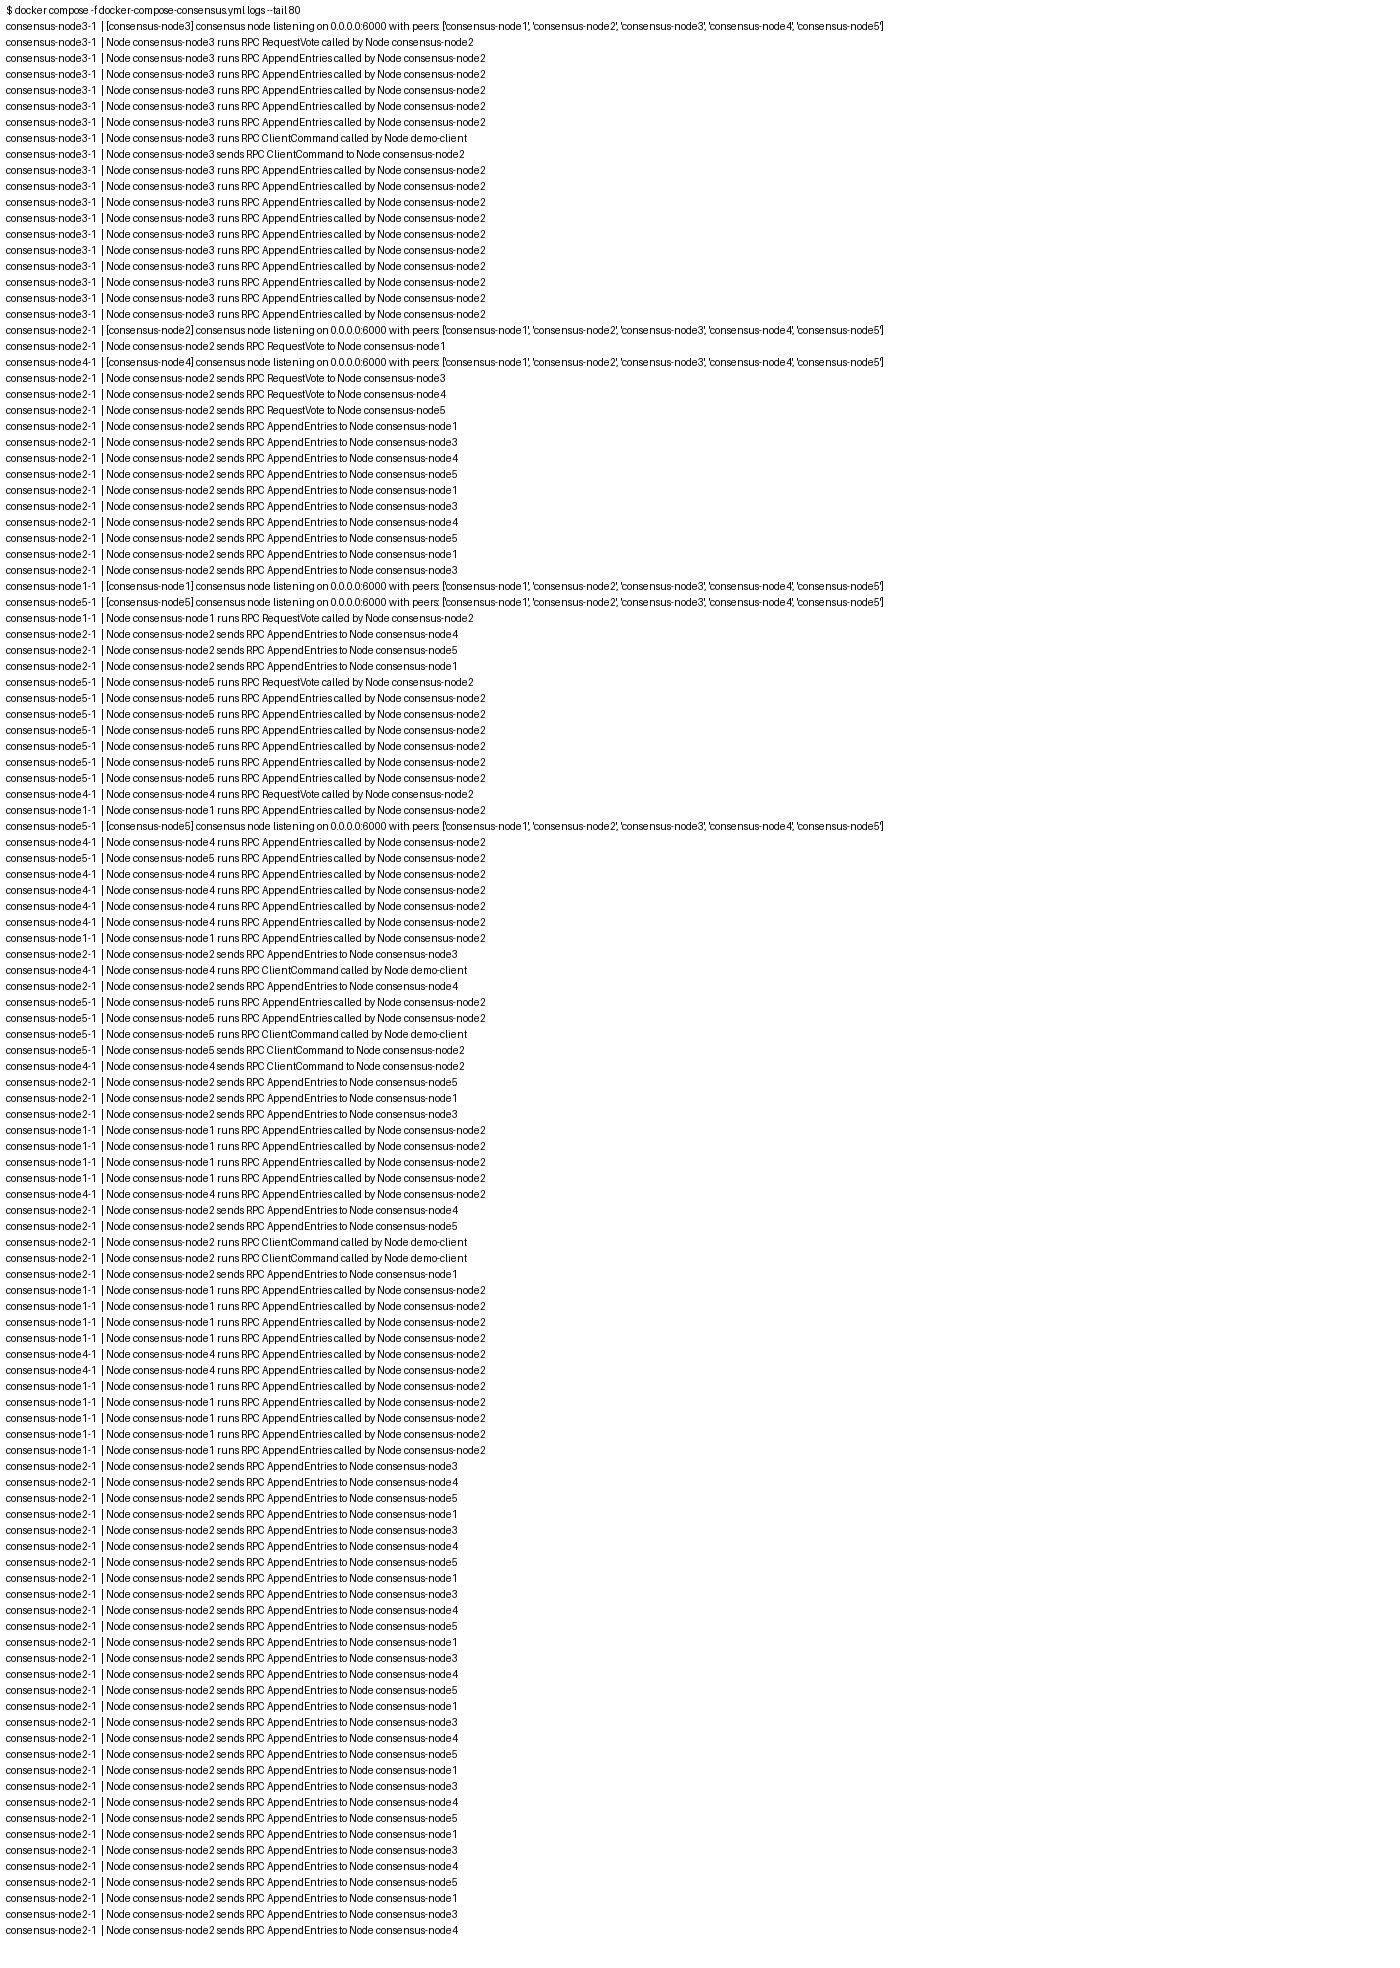
\includegraphics[width=\textwidth]{screenshots/logs_restart_short.png}
  \caption{Leader restart logs}
\end{figure}

\begin{figure}[h]
  \centering
  
\includegraphics[width=0.8\textwidth]{screenshots/store_after_a.png}
  \caption{State after set a 1}
\end{figure}

\begin{figure}[h]
  \centering
  
\includegraphics[width=0.8\textwidth]{screenshots/store_after_b.png}
  \caption{State after set b 2}
\end{figure}

\begin{figure}[h]
  \centering
  
\includegraphics[width=0.8\textwidth]{screenshots/store_after_c.png}
  \caption{State after set c 3 (post-failover)}
\end{figure}

\end{document}
